\documentclass[11.5pt, aspectratio=169]{beamer}
\usepackage{amsmath, amssymb, stmaryrd, mathpartir, commath, url, longtable,hyperref,tabularx}

\usepackage{forloop, microtype}
\usepackage{wasysym}
%\usepackage[dvipsnames]{xcolor}
\usepackage{csquotes}
%\usepackage{mathptmx}
\usepackage{listings}
\hypersetup{colorlinks=true,citecolor=blue}
\RequirePackage{subcaption}
\captionsetup{compatibility=false}
\usepackage{graphicx}
\usepackage{xspace}
\usepackage{dirtytalk}
\usepackage{xparse}% http://ctan.org/pkg/xparse
\usepackage{etoolbox}% http://ctan.org/pkg/etoolbox
\newcommand{\lambdacalc}{\ensuremath{\lambda}-calculus\xspace}
\newenvironment{fake}[1]{\par\vspace{3pt}\noindent\textbf{#1}\itshape}{\normalfont\ignorespacesafterend\vspace{3pt}\par}

\usepackage{float}
\floatstyle{boxed}
\restylefloat{figure}
\usepackage{verbatim}

\newcommand{\backupbegin}{
   \newcounter{finalframe}
   \setcounter{finalframe}{\value{framenumber}}
}
\newcommand{\backupend}{
   \setcounter{framenumber}{\value{finalframe}}
}

\setbeamercovered{%
  again covered={\opaqueness<1->{15}}}



% TIKZ STUFF


\usepackage{amsmath,verbatim}

\lstdefinelanguage{Links}{%
  morekeywords={typename, fun, linfun, op, var, if, this, true, false, else, case, switch, handle,
    handler, shallowhandler, open, do, sig, new, send, receive, spawnAt, spawn,
module, request, accept, try, as, in, otherwise, catch, offer, select, raise,
fork, spawnClient, cancel, catch},%
  sensitive=t, %
  comment=[l]{\#\ },%
  escapeinside={(*}{*)},%
  morestring=[d]{"},%
  keywordstyle=\color{blue},
  showstringspaces=false
  %frame = single
 }

% Links style
\lstset{
  basicstyle=\linespread{1.3}\ttfamily\large,
  keywordstyle=\bfseries,
  language=Links,
  backgroundcolor=\color{white}
}


\usepackage{expl3,xparse}
\makeatletter
\let\old@lstKV@SwitchCases\lstKV@SwitchCases
\def\lstKV@SwitchCases#1#2#3{}
\makeatother
\usepackage{lstlinebgrd}
\makeatletter
\let\lstKV@SwitchCases\old@lstKV@SwitchCases

\lst@Key{numbers}{none}{%
    \def\lst@PlaceNumber{\lst@linebgrd}%
    \lstKV@SwitchCases{#1}%
    {none:\\%
     left:\def\lst@PlaceNumber{\llap{\normalfont
                \lst@numberstyle{\thelstnumber}\kern\lst@numbersep}\lst@linebgrd}\\%
     right:\def\lst@PlaceNumber{\rlap{\normalfont
                \kern\linewidth \kern\lst@numbersep
                \lst@numberstyle{\thelstnumber}}\lst@linebgrd}%
    }{\PackageError{Listings}{Numbers #1 unknown}\@ehc}}
\makeatother

\ExplSyntaxOn
\NewDocumentCommand \lstcolorlines { O{green} m }
{
  \clist_if_in:nVTF { #2 } { \the\value{lstnumber} }{ \color{#1} }{\color{white}}
}
\ExplSyntaxOff
\newcommand{\textl}{\text{\lightning}}


\newcommand{\calcwd}[1]{\mathbf{\mathbf{#1}}}
\newcommand{\one}{\mathbf{1}}
\newcommand{\lightningnu}[1]{\nu #1\lightning}
\newcommand{\gvqueue}[4]{#1(#2){\leftrightsquigarrow} #3(#4)}
\newcommand{\mkwd}[1]{\ensuremath{\mathsf{#1}}}
\newcommand{\gvsend}[2]{\calcwd{send} \: #1 \: #2}
\newcommand{\gvrecv}[1]{\calcwd{receive} \: #1}
\newcommand{\gvcancel}[1]{\calcwd{cancel} \app #1}
\newcommand{\gvclose}[1]{\calcwd{close} \app #1}
\newcommand{\gvcancelup}[1]{\calcwd{cancel} \app #1}
\newcommand{\gvout}[2]{!{#1}.{#2}}
\newcommand{\gvin}[2]{?{#1}.{#2}}
\newcommand{\gvend}{\mathsf{End}\xspace}
\newcommand{\gvfork}[1]{\calcwd{fork} \, #1}
\newcommand{\app}{\:}
\newcommand{\inl}[1]{\calcwd{inl} \app #1}
\newcommand{\inr}[1]{\calcwd{inr} \app #1}
\newcommand{\gvcase}[2]{\calcwd{case} \: #1 \: \calcwd{of} \: \{ #2 \}  }
\newcommand{\gvlet}[3]{\calcwd{let} \: #1 = #2 \: \calcwd{in} \: #3}
\newcommand{\tryasinotherwise}[4]{\calcwd{try} \: #1 \: \calcwd{as} \: #2 \: \calcwd{in} \: #3 \: \calcwd{otherwise} \: #4}
\newcommand{\raiseexn}{\calcwd{raise}\xspace}
\newcommand{\un}[1]{\mkwd{un}(#1)}
\newcommand{\gvdual}[1]{\overline{#1}}
%\newcommand{\compat}{\asymp}
\newcommand{\evalperhaps}{\eval^?}
\newcommand{\evalstar}{\eval^*}
\newcommand{\scancel}[1]{\text{\lightning} #1}
\newcommand{\scancelmv}[1]{#1 \lightning}
\newcommand{\config}[1]{\mathcal{#1}}
\newcommand{\seq}[1]{\overrightarrow{#1}}
\newcommand{\fv}[1]{\mathsf{fv}(#1)}
%\newcommand{\fcv}[1]{\mathsf{fcv}(#1)}
\newcommand{\fvs}[1]{\mathsf{fvs}(#1)}
\newcommand{\fn}[1]{\mathsf{fn}(#1)}
\newcommand{\fcvs}[1]{\fn{#1}}
\newcommand{\chansharp}[1]{#1^{\sharp}}
\newcommand{\chanflat}[1]{#1^{\flat}}
\newcommand{\without}{/}
\newcommand{\equivceval}{\equiv \longrightarrow_{\textsf{C}} \equiv}
\newcommand{\cevalthick}{\Longrightarrow_{\textsf{C}}}
\newcommand{\ceval}{\quad \longrightarrow \quad}
\newcommand{\teval}{\longrightarrow_{\textsf{M}}}
\newcommand{\eps}[1]{\mkwd{eps}(#1)}
\newcommand{\affected}[1]{\mkwd{affected}(#1)}
\newcommand{\halt}{\calcwd{halt}\xspace}
\newcommand{\bcirc}{\bullet}
\newcommand{\wcirc}{\circ}
\newcommand{\disable}[1]{\mkwd{disable}(#1)}

\newcommand{\blocked}[2]{\mkwd{blocked}(#1, #2)}
\newcommand{\depends}[3]{\mkwd{depends}(#1, #2, #3)}
\newcommand{\deadlocked}[1]{\mkwd{deadlocked}(#1)}

\newcommand{\Ceval}{\Longrightarrow_{\textsf{C}}}

\newcommand{\dom}[1]{\mkwd{dom}(#1)}

\newenvironment{remark}{\paragraph{Remark.}}{\hfill \tiny{$\square$}}
%\newtheorem{remark}{Remark}
%\newtheorem{lemma}{Lemma}
%\newtheorem{proposition}{Proposition}
%\newtheorem{corollary}{Corollary}
%\newtheorem{definition}{Definition}


\newcommand{\defeq}{\triangleq}

\newcommand{\todo}[1]{{\noindent\small\color{red} \framebox{\parbox{\dimexpr\linewidth-2\fboxsep-2\fboxrule}{\textbf{TODO:} #1}}}}
\newenvironment{subcase}[1]
  {\textbf{Subcase #1} \hfill \\
  \begin{adjustwidth}{0.25cm}{}}
  {\end{adjustwidth}}

\newenvironment{proofcase}[1]
  {\totheleft{\textbf{Case \textsc{#1}}}}
  {}
\newcommand{\lto}{\multimap}
\newcommand{\proofstep}[1]{
  \begin{compactitem}
  \item #1
  \end{compactitem}
}

\newcommand{\names}[1]{\mkwd{names}(#1)}

\arraycolsep=1pt%\def\arraystretch{2.2}

\newcommand{\transl}[1]{\llbracket #1 \rrbracket}
\newcommand{\stranslateb}[1]{\mathcal{S}\llparenthesis #1 \rrparenthesis}
\newcommand{\ttranslateb}[1]{\mathcal{T}\llparenthesis #1 \rrparenthesis}
\newcommand{\etranslateb}[1]{\mathcal{E}\llparenthesis #1 \rrparenthesis}
\newcommand{\ptranslateb}[1]{\mathcal{P}\llparenthesis #1 \rrparenthesis}

\newcommand{\gvoutone}[1]{{!}#1}
\newcommand{\gvinone}[1]{{?}#1}
\newcommand{\letintwo}[2]{\calcwd{let} \: #1 = #2 \: \calcwd{in}}
\newcommand{\totheleft}[1]{\begin{flushleft}#1\end{flushleft}}
\usepackage[T1]{fontenc}
\usepackage[scaled=0.85]{beramono}
\newcommand\doubleplus{+\kern-1.3ex+\kern0.8ex}
\newcommand{\metadef}[1]{\calcwd{#1}}


\newcommand{\runtimechan}[2]{\mkwd{Channel}(#1, #2)}
\newcommand{\closure}[2]{\langle #1, #2 \rangle}
%\newcommand{\boldleft}{\textbf{\{ }}
%\newcommand{\boldright}{\textbf{ \}}}
\newcommand{\contained}[1]{\metadef{Channels}(#1)}

\newcommand{\ba}{\begin{array}}
\newcommand{\ea}{\end{array}}

\newcommand{\bl}{\ba[t]{@{}l@{}}}
\newcommand{\el}{\ea}


\newcommand{\triestosend}[4]{{#1} \xRightarrow[#4]{#2} {#3}}

\newcommand{\notsmall}{}

\newcommand{\oftype}{\,{:}\,}

\newcommand{\sendpair}[2]{\calcwd{send} \: (#1, #2)}

%\renewcommand{\paragraph}[1]{\textbf{\textit{#1}}}
\usepackage{tikz-cd}

\newcommand{\exnty}{\mkwd{Exn}\xspace}
\newcommand{\raiseexnP}[1]{\calcwd{raise} \: #1}
\newcommand{\tryinunless}[4]{\calcwd{try} \: #1 \: \calcwd{as} \: #2 \:
    \calcwd{in} \: #3 \: \calcwd{unless} \: #4}

\newcommand{\handled}[1]{\mkwd{Handled}(#1)}

\newcommand{\highlight}[1]{{\color{colorredorange} #1} }
\newcommand{\highlightpink}[1]{{\color{colorpink} #1} }
\newcommand{\highlightwarning}[1]{{\color{colorlightpink} #1} }
\newcommand{\midspace}{\; \mid{} \; }
\setlength\tabcolsep{1.5em}

\newcommand{\lact}{\lambda_{\text{act}}\xspace}
\newcommand{\lch}{\lambda_{\text{ch}}\xspace}

\usepackage{config/presento}
\usepackage{framed}
\usepackage{stmaryrd}
\usepackage{amsmath}
\usepackage{wasysym}
% Presento style file
\usepackage{float,lipsum}
\floatstyle{boxed}
\usepackage{mathpartir}
% custom command and packages
% custom packages
\usepackage{textpos}
\setlength{\TPHorizModule}{1cm}
\setlength{\TPVertModule}{1cm}

\newcommand\crule[1][black]{\textcolor{#1}{\rule{2cm}{2cm}}}


\usepackage{verbatim}
% Information
\title{Model-View-Update, and Beyond!}
\subtitle{Adventures in Formalising and Extending the Elm Architecture}
\author{Simon Fowler}
\institute{University of Edinburgh}
\date{12th March 2019}

\begin{document}

% Title page
\begin{frame}[plain]
\titlepage


\hfill
\vspace{-1em}
$
\renewcommand*{\arraystretch}{1.8}
\begin{array}{r}
   
\includegraphics[height=0.7cm, keepaspectratio]{images/logos/inf_uoe.png} \\
\end{array}
$
\end{frame}
\begin{frame}{Links: Web Programming without Tiers}

  \centering
  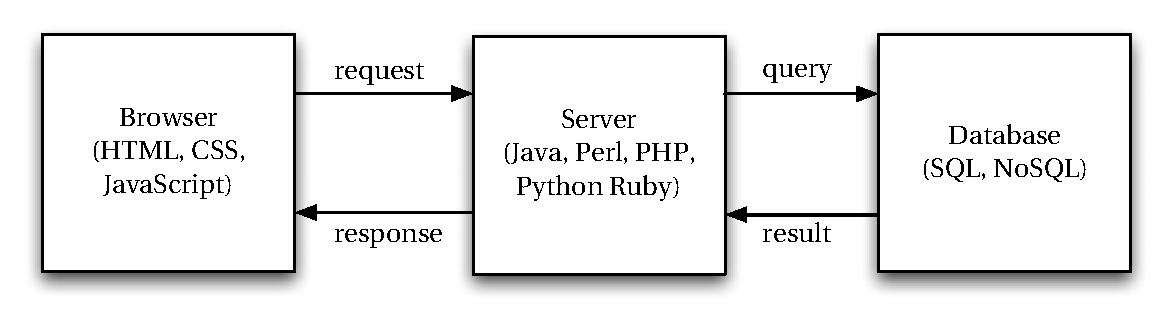
\includegraphics[width=0.5\paperwidth]{images/3tier.pdf}
  \vspace{1em}

  \begin{fullpageitemize}
    \itemR \textbf{Idea}: Uniform language for ``tierless'' web programming: client, server, DB code all in same language (Cooper et al., 2006)
    \itemR Statically-typed, ML-inspired, impure functional language
    \itemR With \emph{lots} of cool research features
  \end{fullpageitemize}
  \vspace{1em}
\end{frame}

\begin{frame}{Minimal Example: A Box and a Label}
  \begin{center}
    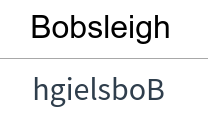
\includegraphics[scale=0.5]{images/label.png}
  \end{center}

  \begin{fullpageitemize}
  \itemR Very small illustrative example
  \itemR Text contained in a \texttt{div} should reflect value of a form input box, reversed
  \end{fullpageitemize}
\end{frame}


\begin{frame}[fragile]{Vanilla Links Implementation}
%fun getProp(id, propName) { ... }
%fun setProp(id, propName, newVal) { ... }
  \begin{lstlisting}[language=links]
fun mainPage() {
  fun handleEvents() {
    receive { case UpdateLabel ->
      var value = getProp("toReverse", "value");
      setProp("label", "innerHTML", reverseString(value));
      handleEvents()
    }
  }
  var evtHandler = spawnClient { handleEvents() };
  page
    <html>
      <body>
        <form>
          <input type="text" id="toReverse"
            l:onkeyup="{evtHandler ! UpdateLabel}"></input>
        </form>
        <div id="label"></div>
      </body>
    </html>
}
  \end{lstlisting}
\end{frame}

\begin{frame}{Vanilla Links Model}

  \begin{center}
     % TODO: Diagram (TiKZ?)
    \begin{tikzpicture}[node distance=1.5cm]
      \node (0) [diagnode] { Event invoked };
      \node (1) [diagnode, below of=0]{ Message sent to handler };
      \node (2) [diagnode, below of=1]{ Process reads data from DOM };
      \node (3) [diagnode, below of=2]{ Process updates data in DOM };

      \draw [arrow] (0) -- (1);
      \draw [arrow] (1) -- (2);
      \draw [arrow] (2) -- (3);
    \end{tikzpicture}
  \end{center}

  \begin{fullpageitemize}
  \itemR \textbf{Depressingly} imperative
    \begin{itemize}
  \itemR DOM is essentially one big chunk of mutable state
  \itemR Explicit retrieval from / mutation of DOM elements
  \end{itemize}
  \end{fullpageitemize}
\end{frame}


\framecard{{\color{white}\bigtext{Model-View-Update, or The Elm Model}}}

\begin{frame}{The Elm Programming Language}

  \begin{center}
    
\includegraphics[width=0.5\textwidth]{images/ElmLogo.png}
  \end{center}

  \begin{fullpageitemize}
  \itemR Statically-typed, Haskell-esque, purely-functional programming language, geared towards web programming
  \itemR Originally based on applicative functional reactive programming
    \begin{itemize}
      \itemR \ldots however the designers later (correctly) realised that message passing was a better fit
      \itemR Pioneers the \emph{model-view-update} pattern
    \end{itemize}
  \end{fullpageitemize}

\end{frame}

\begin{frame}[fragile]{Links-MVU: A Box and a Label}
\begin{lstlisting}[language=Links]
typename Model = (contents: String);
typename Message = [| UpdateBox: String |];

fun updt(UpdateBox(newStr), model) { newStr }

fun view(model) {
  var a0 = MvuAttrs.empty; var h0 = MvuHTML.empty;
  div(a0, form(a0,
      input(type("text") +@
            onKeyUp(fun(str) { UpdateBox(str) }), h0)) +*
    div(a0, textNode(reverseString(model.contents))))
}

fun mainPage() {
  Mvu.runSimple("placeholder", (contents=""), view, updt);
  page <html><body><div id="placeholder"></div></body></html>
}
\end{lstlisting}
\end{frame}

\begin{frame}[fragile]{The Essence of the Elm Architecture}

  \begin{fullpageitemize}
  \item<1-> User-defined types:
    \begin{itemize}
      \itemR Model type \verb+Model+, containing application data
      \itemR Message type \verb+Msg+, describing messages produced by components
    \end{itemize}
    \vspace{0em}

  \item<2-> HTML type \verb+HTML(Msg)+: an HTML element producing a message of
    type \verb+Msg+

  \item<3-> A function, \verb+run+:
    \begin{verbatim}
      run: forall model, msg.
        (model,                          // Initial model
         (model) -> HTML(msg),           // View function
         (model, msg) ~> model)          // Update function
        ~> ()
    \end{verbatim}

    \vspace{0em}

  \item<4-> HTML generated by \verb+Render+ \emph{diffed} against current DOM, lightweight updates
  \item<5-> (Also \emph{subscriptions} which allow events like time, mouse movement
    to generate messages---omitted here for simplicity)
  \end{fullpageitemize}
\end{frame}

\begin{frame}[fragile]{Implementing the Elm Architecture in Links}

  \begin{minipage}{0.475\textwidth}
  \begin{lstlisting}[language=links]
fun evtLoop(model, render, updt) {
  receive {
    case msg ->
      var newModel = updt(msg, model);
      # Update DOM
      VDom.updateDom(
        render(newModel));
      # Loop with new model
      evtLoop(newModel, render, updt)
    }
}
\end{lstlisting}
\end{minipage}
~\hfill
\begin{minipage}{0.5\textwidth}
\begin{lstlisting}[language=JavaScript]
function _updateDom(doc) {
  var newTree = jsonToVtree(doc);
  var patches =
    diff(currentVDom, newTree);
  currentVDom = newTree;
  rootNode =
    patch(rootNode, patches);
}
\end{lstlisting}
\end{minipage}

  \begin{fullpageitemize}
  \item Implementation with Jake Browning, LFCS intern, over summer 2017
  \item Made use of typed actor-style concurrency in Links (since updated)
  \item Required implementation of JS FFI
  \end{fullpageitemize}
\end{frame}

\begin{frame}{Real applications!}

  \begin{center}
    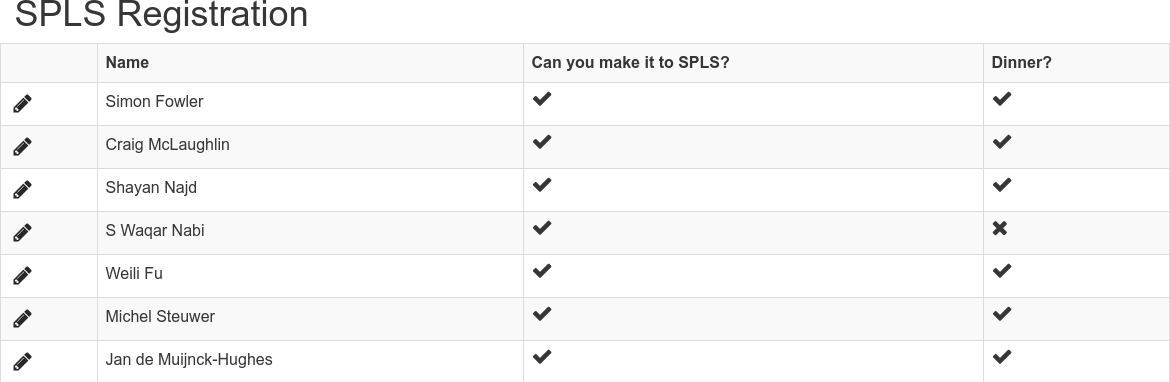
\includegraphics[width=0.75\textwidth]{images/spls-reg.png}
  \end{center}

  \begin{itemize}
    \itemR Also TodoMVC, Pong, a few more\ldots
  \end{itemize}
\end{frame}


\begin{frame}{Two questions}
  \begin{fullpageitemize}
  \item {\Large \textbf{What would be a sensible formal model for MVU?}}
    \begin{itemize}
      \itemR Formal model would make the paradigm more precisely-defined and easier to implement in future
    \end{itemize}
    \vspace{1em}
  \item {\Large \textbf{Can we use MVU to write web applications with distributed session types?}}
    \begin{itemize}
      \itemR Writing client code using distributed session-typed channels in Links is painful: can we do better?
    \end{itemize}
  \end{fullpageitemize}
\end{frame}

\framecard{{\color{white}\bigtext{Formalising MVU}}}

\begin{frame}{Key concepts}

  \begin{fullpageitemize}
  \item {\Large \textbf{Reactivity}}
    \begin{itemize}
      \itemR Computation is driven by external events (for example, a button being clicked)
    \end{itemize}
    \vspace{0.5em}
  \item {\Large \textbf{Typed HTML and antiquotations}}
    \begin{itemize}
      \itemR HTML is typed and first class
      \itemR Terms can be spliced into HTML elements and attributes
    \end{itemize}
    \vspace{0.5em}
  \item {\Large \textbf{Concurrency}}
    \begin{itemize}
      \itemR Naturally concurrent: modelled by a concurrent $\lambda$-calculus (with actor-style concurrency)
    \end{itemize}
  \end{fullpageitemize}
\end{frame}

\begin{frame}{Formalism by Example}

  \begin{mathpar}
    \mkwd{model} \defeq "h"

    \mkwd{updt} \defeq \lambda (\text{msg}, \text{model}) . \text{msg}
  \end{mathpar}


  \[
    \bl
    \mkwd{view} \defeq \lambda \textit{contents} . \\
    \quad
      \ot{div} \\
      \qquad \ot{form} \\
      \quad \qquad \htmltag{input}{\attr{id}{1} \; \attr{type}{"text"} \;
      \attr{onInput}{\antiquote{\lambda x . x}}}{} \\
      \quad \qquad \htmltag{div}{\attr{id}{2}}{\antiquote{\mkwd{reverseString}(\textit{contents})}} \\
      \qquad \ct{form} \\
    \quad
      \ct{div} \\
    \el
  \]
\end{frame}

\begin{frame}{Formalism by Example}

  \begin{mathpar}
    \mkwd{model} \defeq "h"

    \mkwd{updt} \defeq \lambda (\text{msg}, \text{model}) . \text{msg}
  \end{mathpar}


  \[
    \bl
    \mkwd{view} \defeq \lambda \textit{contents} . \\
    \quad
      \ot{div} \\
      \qquad \ot{form} \\
      \quad \qquad \htmltag{input}{\attr{id}{1} \; \attr{type}{"text"} \; \attr{value}{\antiquote{\textit{contents}}} \;
        \attr{onInput}{\antiquote{\lambda x . x}}}{} \\
      \quad \qquad \htmltag{div}{\attr{id}{2}}{\antiquote{\mkwd{reverseString}(\textit{contents})}} \\
      \qquad \ct{form} \\
    \quad
      \ct{div} \\
    \el
  \]
\end{frame}

\begin{frame}{Formalism by Example}
  \[
    \vh \defeq
    \bl
      \ot{div} \\
      \quad \ot{form} \\
      \qquad \htmltag{input}{\attr{id}{1} \; \attr{type}{"text"} \; \attr{value}{"h"} \; \attr{onInput}{\lambda x . x}}{} \\
      \qquad \htmltag{div}{\attr{id}{2}}{h} \\
      \quad \ct{form} \\
      \ct{div} \\
    \el
  \]

  \only<1>{
    {
      \Large
    \[
    \sys{\handlerproc{\idle}{"h"}{\mkwd{view}}{\mkwd{updt}}{\epsilon}}{\vh}{\epsilon}{\epsilon}
    \]
    }
  }

 \only<2>{
   {
     \Large
   \[
     \sys{\handlerproc{\idle}{"h"}{\mkwd{view}}{\mkwd{updt}}{\epsilon}}{\vh}{\epsilon}{\clickevt{1}}
   \]
   }
 }
%
  \only<3>{
    {
      \Large
    \[
      \sys{\handlerproc{\idle}{"h"}{\mkwd{view}}{\mkwd{updt}}{\epsilon}}{\vh}{\epsilon}{\clickevt{1}}
    \]
    }
    \[
      \vh(1, \mkwd{onClick}) \text{ undefined}
    \]
  }

  \only<4>{
    {
      \Large
    \[
      \sys{\handlerproc{\idle}{"h"}{\mkwd{view}}{\mkwd{updt}}{\epsilon}}{\vh}{\epsilon}{\epsilon}
    \]
    }
  }
%
%
 \only<5>{
   {
     \Large
   \[
     \sys{\handlerproc{\idle}{"h"}{\mkwd{view}}{\mkwd{updt}}{\epsilon}}{\vh}{\epsilon}{\inputevt{1}{"hi"}}
   \]
   }
 }

 \only<6>{
   {
   \Large
   \[
     \sys{\handlerproc{\idle}{"h"}{\mkwd{view}}{\mkwd{updt}}{\epsilon}}{\vh}{(\lambda x . x) \app "hi"}{\epsilon}
   \]
   }
   %
   \[
     \vh(1, \mkwd{onInput}) = \lambda x . x
   \]
 }

 \only<7>{
   {
   \Large
   \[
     \sys{\handlerproc{\idle}{"h"}{\mkwd{view}}{\mkwd{updt}}{\epsilon}}{\vh}{"hi"}{\epsilon}
   \]
   }
 }

 \only<8>{
   {
   \Large
   \[
     \sys{\handlerproc{\idle}{"h"}{\mkwd{view}}{\mkwd{updt}}{"hi"}}{\vh}{\epsilon}{\epsilon}
   \]
   }
 }

 \only<9>{
   {
   \Large
   \[
     \sys{\handlerproc{
         {\normalsize
         \begin{array}{l}
           \begin{aligned}
             & \letintwo{m'}{(\lambda (\textit{model}, \textit{msg}). \textit{msg}) \app ("\text{h}", "\text{hi}")} \\
             & (m', v \app m')
           \end{aligned}
         \end{array}
       }
     }{"h"}{\mkwd{view}}{\mkwd{updt}}{\epsilon}}{\vh}{\epsilon}{\epsilon}
   \]
   }
 }

 \only<10>{
   {
   \Large
   \[
     \sys{\handlerproc{
         {\normalsize
         \begin{array}{l}
           \begin{aligned}
             & \letintwo{m'}{"\text{hi}"} \\
             & (m', v \app m')
           \end{aligned}
         \end{array}
       }
     }{"h"}{\mkwd{view}}{\mkwd{updt}}{\epsilon}}{\vh}{\epsilon}{\epsilon}
   \]
   }
 }

 \only<11>{
   {
   \Large
   \[
     \sys{\handlerproc{
         {\normalsize
           ("\text{hi}", v \app "\text{hi}")
       }
     }{"h"}{\mkwd{view}}{\mkwd{updt}}{\epsilon}}{\vh}{\epsilon}{\epsilon}
   \]
   }
 }

\end{frame}

\begin{frame}{Formalism by Example}

  \only<1>{
   \Large
   \[
     \sys{\handlerproc{
    {\small
      ("\text{hi}", \bl
      (\lambda \text{contents}. \\
    \quad \ot{div} \\
      \qquad \ot{form} \\
      \quad \qquad \htmltag{input}{\attr{id}{1} \; \attr{type}{"text"} \; \\
        \qquad \qquad
      \attr{value}{\antiquote{\textit{contents}}}{} \\
        \qquad \qquad
      \attr{onInput}{\antiquote{\lambda x . x}}}{} \\
      \quad \qquad \opentag{div}{\attr{id}{2}} \\
         \qquad \qquad
       \antiquote{\mkwd{reverseString}(\textit{contents})} \\
       \quad \qquad \closetag{div} \\
      \qquad \ct{form} \\
    \quad
    \ct{div} ) \app "\text{hi}" \\
    \el
    )
  }
   }{"h"}{\mkwd{view}}{\mkwd{updt}}{\epsilon}}{\vh}{\epsilon}{\epsilon}
  \]
  }
%
  \only<2>{
   \Large
   \[
     \sys{\handlerproc{
    {\small
      ("\text{hi}", \bl
    \ot{div} \\
      \quad \ot{form} \\
      \qquad \htmltag{input}{\attr{id}{1} \; \attr{type}{"text"} \; \\
        \quad \qquad
      \attr{value}{\antiquote{"\text{hi}"}}{} \\
        \quad \qquad
      \attr{onInput}{\antiquote{\lambda x . x}}}{} \\
      \qquad \opentag{div}{\attr{id}{2}} \\
         \quad \qquad
       \antiquote{\mkwd{reverseString}("\textit{hi}")} \\
       \qquad \closetag{div} \\
      \quad \ct{form} \\
    \ct{div} \\
    \el)
  }
   }{"h"}{\mkwd{view}}{\mkwd{updt}}{\epsilon}}{\vh}{\epsilon}{\epsilon}
  \]
  }
%
  \only<3>{
   \Large
   \[
     \sys{\handlerproc{
    {\small
      ("\text{hi}", \bl
    \ot{div} \\
      \quad \ot{form} \\
      \qquad \htmltag{input}{\attr{id}{1} \; \attr{type}{"text"} \; \\
        \quad \qquad
      \attr{value}{"\text{hi}"}{} \\
        \quad \qquad
      \attr{onInput}{\antiquote{\lambda x . x}}}{} \\
      \qquad \opentag{div}{\attr{id}{2}} \\
         \quad \qquad
       \antiquote{\mkwd{reverseString}("\textit{hi}")} \\
       \qquad \closetag{div} \\
      \quad \ct{form} \\
    \ct{div} \\
    \el)
  }
   }{"h"}{\mkwd{view}}{\mkwd{updt}}{\epsilon}}{\vh}{\epsilon}{\epsilon}
  \]
  }
%
  \only<4>{
   \Large
   \[
     \sys{\handlerproc{
    {\small
      ("\text{hi}", \bl
    \ot{div} \\
      \quad \ot{form} \\
      \qquad \htmltag{input}{\attr{id}{1} \; \attr{type}{"text"} \; \\
        \quad \qquad
      \attr{value}{"\text{hi}"}{} \\
        \quad \qquad
      \attr{onInput}{\lambda x . x}}{} \\
      \qquad \opentag{div}{\attr{id}{2}} \\
         \quad \qquad
       \antiquote{\mkwd{reverseString}("\textit{hi}")} \\
       \qquad \closetag{div} \\
      \quad \ct{form} \\
    \ct{div} \\
    \el)
  }
   }{"h"}{\mkwd{view}}{\mkwd{updt}}{\epsilon}}{\vh}{\epsilon}{\epsilon}
  \]
  }
%
  \only<5>{
   \Large
   \[
     \sys{\handlerproc{
    {\small
      ("\text{hi}", \bl
    \ot{div} \\
      \quad \ot{form} \\
      \qquad \htmltag{input}{\attr{id}{1} \; \attr{type}{"text"} \; \\
        \quad \qquad
      \attr{value}{"\text{hi}"}{} \\
        \quad \qquad
      \attr{onInput}{\lambda x . x}}{} \\
      \qquad \opentag{div}{\attr{id}{2}} \antiquote{"\textit{ih}"} \closetag{div} \\
      \quad \ct{form} \\
    \ct{div} \\
    \el)
  }
   }{"h"}{\mkwd{view}}{\mkwd{updt}}{\epsilon}}{\vh}{\epsilon}{\epsilon}
  \]
  }
%
  \only<6>{
   \Large
   \[
     \sys{\handlerproc{
    {\small
      ("\text{hi}", \bl
    \ot{div} \\
      \quad \ot{form} \\
      \qquad \htmltag{input}{\attr{id}{1} \; \attr{type}{"text"} \; \\
        \quad \qquad
      \attr{value}{"\text{hi}"}{} \\
        \quad \qquad
      \attr{onInput}{\lambda x . x}}{} \\
      \qquad \opentag{div}{\attr{id}{2}} \textit{ih} \closetag{div} \\
      \quad \ct{form} \\
    \ct{div}  \\
    \el)
  }
   }{"h"}{\mkwd{view}}{\mkwd{updt}}{\epsilon}}{\vh}{\epsilon}{\epsilon}
  \]
  }
%
  \only<7>{
   \Large
   \[
     \sys{\handlerproc{\idle}{"hi"}{\mkwd{view}}{\mkwd{updt}}{\epsilon}}{
       {\small
      \bl
        \ot{div} \\
          \quad \ot{form} \\
          \qquad \htmltag{input}{\attr{id}{1} \; \attr{type}{"text"} \; \\
            \quad \qquad
          \attr{value}{"\text{hi}"}{} \\
            \quad \qquad
          \attr{onInput}{\lambda x . x}}{} \\
          \qquad \opentag{div}{\attr{id}{2}} \textit{ih} \closetag{div} \\
          \quad \ct{form} \\
        \ct{div}  \\
        \el
      }
     }{\epsilon}{\epsilon}
  \]
  }
\end{frame}

\begin{frame}{Syntax}

    \small
    \begin{syntax}
      \text{Types} & A, B & ::= & \one \midspace A \to B \midspace A \times B  \midspace A + B \midspace \htmlty{A} \midspace C \\
    \text{Base types} & C & ::= & \mkwd{String} \midspace \mkwd{Int} \midspace \mkwd{Bool} \\ \\
    \text{String literals} & s \\
    \text{Integers} & n \\
    \text{Booleans} & b & ::= & \ttrue \midspace \ffalse \\
    \text{Terms} & L, M, N & ::= &
      % Basic lambda calculus
      x \midspace \lambda x . M \midspace M \app N \midspace () \midspace (M, N) \midspace \letin{(x, y)}{M}{N} \\
      & & \midspace & \inl{M} \midspace \inr{M} \midspace \caseof{L}{\inl{x} \mapsto M; \inr{y} \mapsto N} \\
      & & \midspace & s \midspace n \midspace b \midspace \htmlterm{H} \\
      \\
    \text{Tag names} & \tagname{t} \\
    \text{Attribute names} & \mathit{at} \\
    \text{Event handlers} & \mkwd{eh} & ::= &
      \texttt{onClick} \midspace \texttt{onKeyDown} \midspace \texttt{onKeyUp} \\
      \text{Attributes} & a & ::= & \mkwd{id} = n \midspace \mkwd{eh} = \textit{ab} \midspace  \textit{at} = \textit{ab}\\
      \text{Attribute bodies} & \textit{ab} & ::= & \antiquote{M} \midspace V \\
      \text{HTML} & H & ::= & \htmltag{t}{\seq{a}}{\seq{H}} \midspace s  \midspace \antiquote{M} \\
\end{syntax}
\end{frame}

\begin{frame}{Typing Judgements}

  \begin{center}
  {\Huge \framebox{$\Gamma \vdash M : A$}}
  \vspace{0.5em}

    ``Under environment $\Gamma$, term $M$ has type $A$.''
  \end{center}
  \vspace{1em}

  \begin{center}
  {\Huge \framebox{$\Gamma \vdash a \produces{A}$}}
  \vspace{0.5em}

    ``Under environment $\Gamma$, HTML attribute $a$ produces messages of type $A$.''
  \end{center}
  \vspace{1em}

  \begin{center}
  {\Huge \framebox{$\Gamma \vdash H \produces{A}$}}
  \vspace{0.5em}

    ``Under environment $\Gamma$, HTML element $a$ produces messages of type $A$.''
  \end{center}
\end{frame}

\begin{frame}{Results}

  {\large
\begin{theorem}[Preservation (Configurations)]
  \label{thm:config-pres}
  If $\Gamma \vdash \config{C}$ and $\config{C} \ceval \config{D}$, then $\Gamma \vdash \config{D}$.
\end{theorem}
%
\vspace{2em}
%
  \begin{theorem}[Event Progress]\label{thm:event-progress}
    If $\cdot \vdash \config{C}$, then either:
    \begin{itemize}
      \itemR $\config{C}$ can be written $\sys{\handlerproc{\idle}{V_m}{V_v}{V_u}{\epsilon}}{\vh}{\epsilon}{\epsilon}$; or
      \itemR there exists some $\config{C}'$ such that $\config{C} \ceval \config{C'}$.
      \end{itemize}
  \end{theorem}
}
\end{frame}


\framecard{{\color{white}\bigtext{MVU + Distributed Session Types}}}

\begin{frame}{Linear Messages and Models}

  \begin{center}
    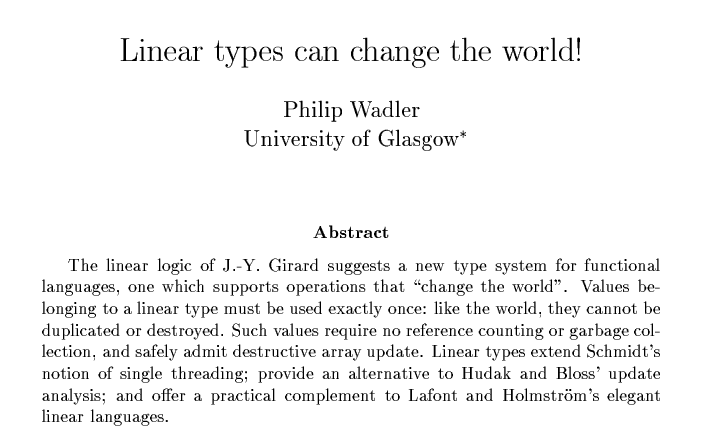
\includegraphics[width=0.6\textwidth]{images/linear-types.png}
  \end{center}

  \begin{fullpageitemize}
  \item \textbf{Linear Type Systems}: Ensure variables are used \emph{exactly once}
  \begin{itemize}
    \itemR Useful for resource tracking, functional in-place update of arrays, quantum programming languages\ldots
  \end{itemize}
  \end{fullpageitemize}

\end{frame}

\begin{frame}[fragile]{Session Types in Links}

\begin{lstlisting}[language=links]
  typename EqualityServer = ?Int.?Int.!Bool.End;

  sig equalityServer : (EqualityServer) ~> ()
  fun equalityServer(s) {
    var (x, s) = receive(s);
    var (y, s) = receive(s);
    var s = send(x == y, s);
    close(s)
  }
\end{lstlisting}
\end{frame}

\begin{frame}[fragile]{Session Types}
\begin{lstlisting}[language=links]
  typename EqualityServer = ?Int.?Int.!Bool.End;

  sig equalityServer : (EqualityServer) ~> ()
  fun equalityServer(s) {
    var (x, t) = receive(s);
    (*\hlred{var (y, s) = receive(s);} *)
    var (z, s) = receive(s);
    var s = send(x == y, s);
    close(s)
  }
\end{lstlisting}
\end{frame}

\begin{frame}[fragile]{Can MVU support linearity?}

  \begin{fullpageitemize}
  \item We want \emph{linear models and messages}.
    \begin{itemize}
      \itemR but\ldots
    \end{itemize}
  \end{fullpageitemize}

  \begin{lstlisting}[language=links]
fun evtLoop(updt, render, model) {
  receive {
    case msg ->
      var newModel = updt(msg, model);
      # Update DOM
      VDom.updateDom(render((*\color{red}{newModel}*)));
      # Loop with new model
      evtLoop(updt, render, (*\color{red}{newModel}*))
    }
}
  \end{lstlisting}

  \begin{fullpageitemize}
    \item \texttt{newModel} is used twice, violating linearity!
  \end{fullpageitemize}
\end{frame}

\begin{frame}[fragile]{MVU with Linearity (1)}

\begin{minipage}{0.55\textwidth}
  \begin{lstlisting}[language=links]
fun evtLoop(ap, model, render, updt, extract) {
  var (msg, _) = receive(request(ap));
  var newModel = updt(msg, model);
  # Update DOM
  var (html, newModel) =
    render(unrModel);
  VDom.updateDom(html);
  # Loop with new model
  evtLoop(newModel, render, updt, extract)
}
  \end{lstlisting}
\end{minipage}
~
\begin{minipage}{0.42\textwidth}
  \begin{lstlisting}[numbers=none, backgroundcolor=\color{white}]
runLinear :
 forall model::Type(Any, Any),
        msg::Type(Any, Any) .
 (model,
   (*\texttt{\textbf{\color{colorredorange}{(model) -> (HTML(msg), model)}}}*),
   (model, msg) ~> (model))
  ~> ()
\end{lstlisting}
\end{minipage}

  \begin{fullpageitemize}
  \item ``Standard'' way of generalising an unrestricted function: return an `updated' linear resource
  \item Works, but breaks abstraction: rendering can in turn update model
   %\begin{itemize}
   %  \item In our setting, could also perform session communication while rendering: is this what we want?
   %\end{itemize}
  \end{fullpageitemize}
\end{frame}

\begin{frame}[fragile]{MVU with Linearity (2)}

\begin{minipage}{0.55\textwidth}
  \begin{lstlisting}[language=links]
fun evtLoop(ap, model, render, updt, extract) {
  var (msg, _) = receive(request(ap));
  var newModel = updt(msg, model);
  # Extract unrestricted model
  (*\texttt{\textbf{\color{colorredorange}{var (newModel, unrModel) = extract(newModel);}}} *)
  # Update DOM
  VDom.updateDom(render(unrModel));
  # Loop with new model
  evtLoop(newModel, render, updt, extract)
}
  \end{lstlisting}
\end{minipage}
~
\begin{minipage}{0.42\textwidth}
\begin{verbatim}
runLinear :
  forall model :: Type(Any, Any),
         unrModel :: Type(Unl, Any),
         msg :: Type(Any, Any) .
  (model,
   (unrModel) ~> HTML(msg),
   (model, msg) ~> (model),
   (model) ~> (model, unrModel))
  ~> ()
\end{verbatim}
\end{minipage}

  \begin{fullpageitemize}
  \item \textbf{Observation:} The linear model is required in the \texttt{updt} function, but \emph{only unrestricted data} is used when rendering the webpage
    \begin{itemize}
      \itemR An \texttt{extract} function extracts the unrestricted part of a model, which is passed to the rendering function
    \end{itemize}
  \end{fullpageitemize}
\end{frame}

\framecard{{\color{white}\bigtext{Demo: Session-typed Distributed Chat}}}


\begin{frame}{Session Types in Links}
\end{frame}

\begin{frame}{Distributed Session Types}
\end{frame}

\begin{frame}{Linearity meets MVU}
\end{frame}

\begin{frame}{Session-typed communication meets MVU}
\end{frame}

\begin{frame}{A nontrivial application}
\end{frame}

\framecard{{\color{white}\bigtext{Wrapping up}}}

\begin{frame}{The future}
  \begin{fullpageitemize}
    \item {\large \textbf{Formalising Extensions}}
    \item {\large \textbf{Small-step interpreter}}
  \end{fullpageitemize}
\end{frame}

\begin{frame}{Conclusion}
\end{frame}

\end{document}

